\subsection{K-Means}
We have tested on each dataset 57 different configurations of the K-Means algorithm, by using the 3 different distance metrics with 19 different values of the k (from 2 to 20). For each of these configurations, we have run the K-Means 10 times, in order to account for the randomness of the centroid initialization. This results in a total of 570 runs of the K-Means algorithm for each dataset. From the evaluation metrics extracted for each of these runs, we study the effect of each of the 2 hyperparameters and study the best performing runs according to each of the metrics.

\subsubsection{Hyperparameter Study}
First of all, let us start by observing some preliminary patterns about the measured metrics and the effect of each hyperparameter on the clustering performance.

In Figure \ref{fig:metrics_corr} we summarize the relationship between the different metrics that were measured for two datasets. Each is a matrix plot where the lower triangle is a heatmap of the Pearson correlations between each pair of metrics, the diagonal elements are the histogram distributions of values of each metric, and the upper triangular has for each pair of metrics the plot of their values for all runs. It is interesting to observe that, while we would expect all of the metrics to agree on the identified trends, there are some cases where the opposite behavior is displayed in each dataset. We observe that most of the strongest correlations are preserved (NMI-ARI, Silhouette-DBI, CHS-Silhouette), but others are completely reversed (DBI-ARI, CHS-NMI). This could be due to changes in the hyperparameters which interact differently with the metrics, depending on the nature of the dataset.

\begin{figure}[h!]
    \centering
    \begin{subfigure}{0.49\textwidth}
        \centering
        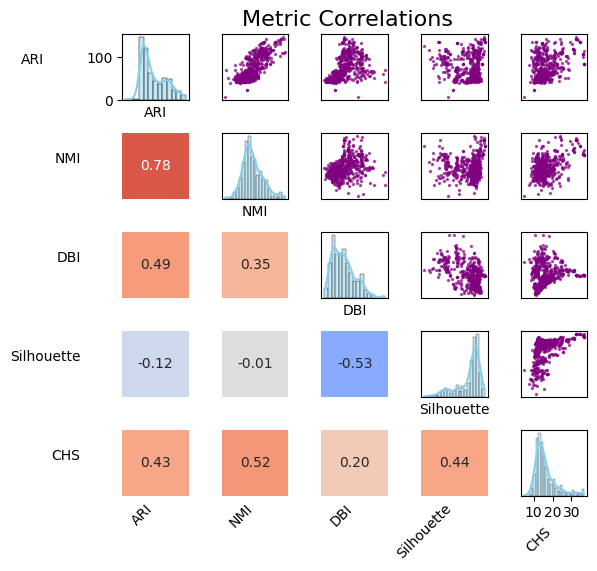
\includegraphics[width=\linewidth]{figures/KMeans/hepatitis_metrics_correlations_matrix.png}
        \caption{Hepatitis metric correlations}
    \end{subfigure}
    \hfill
    \begin{subfigure}{0.49\textwidth}
        \centering
        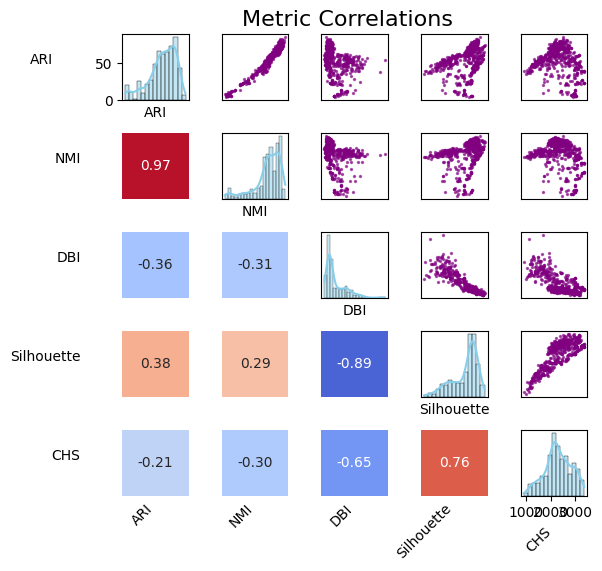
\includegraphics[width=\linewidth]{figures/KMeans/penbased_metrics_correlations_matrix.png}
        \caption{Pen-based metric correlations}
    \end{subfigure}
    \caption{Metric correlations and distributions in two datasets}
    \label{fig:metrics_corr}
\end{figure}

Parallelly, a different set of interesting relationship are displayed in Figure \ref{fig:pairplot}, where we can see heatmaps of the ARI and the Time across the different pairwise hyperparameter configurations. We can observe a general trend regarding execution time: it seems to have considerably larger values for the Clark distance metric compared to those of the other 2, which reflects the higher computational cost that this distance metric has. Additionally, we see a noteworthy divergence in the ARI trends: in the Hepatitis dataset (which has 2 classes), lower values of k seem to achieve a better ARI, with a significantly better performance with the Clark distance metric than with the other two; meanwhile, in the Pen-based dataset (which has 10 classes), bigger values of k ($>$7) seem to achieve the best scores, with a somewhat lower performance with the Clark distance than with the other two. The behavior with respect to the k was to be expected due to the true number of labels of each dataset, yet it still is compelling to see it reflected so clearly in the results. On the other hand, it is enlightening to see opposite behaviors with respect to the distance metric, which reflects that the Clark distance fails to capture some intrinsic properties of the Pen-based dataset, while it excells to do so within the Hepatitis dataset.

\begin{figure}[H]
    \centering
    \begin{subfigure}{0.49\textwidth}
        \centering
        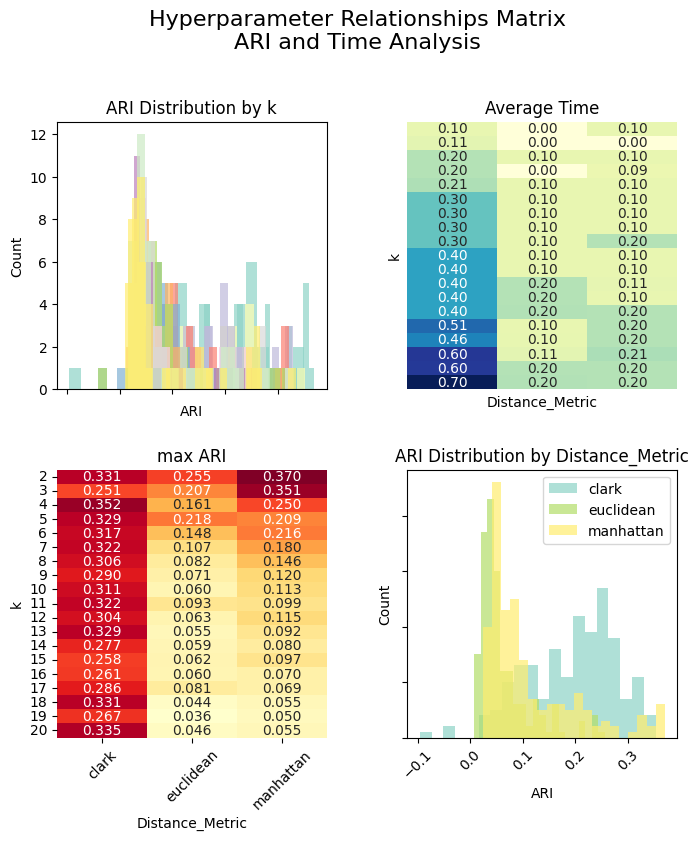
\includegraphics[width=\linewidth]{figures/KMeans/hepatitis_hyperparameter_pairplot_matrix.png}
        \caption{Hepatitis pairplot matrix}
    \end{subfigure}
    \hfill
    \begin{subfigure}{0.49\textwidth}
        \centering
        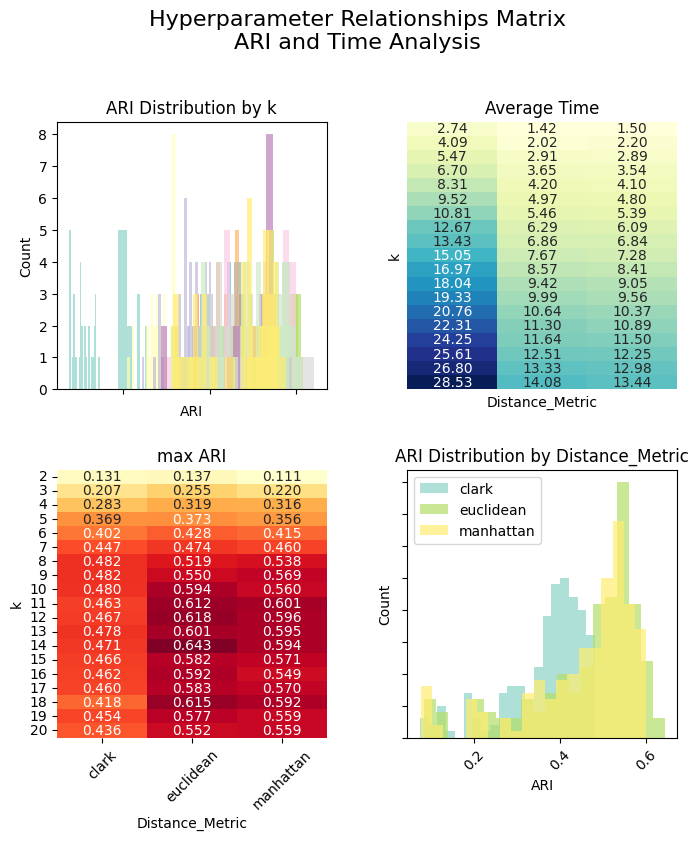
\includegraphics[width=\linewidth]{figures/KMeans/penbased_hyperparameter_pairplot_matrix.png}
        \caption{Pen-based pairplot matrix}
    \end{subfigure}
    \caption{Hyperparameter pairplot matrices based on F1 Score and Time}
    \label{fig:pairplot}
\end{figure}

We can clearly observe the trends regarding the value of k in the violin plot in Figure \ref{fig:kmeans:violin}. This time, for Hepatitis and Pen-based we plot the NMI metric, which again shows the same behavior: in Hepatitis, we observe a clear maximum of consistency for k=2, and then a constant decrease in performance as k increases; while, in Pen-based, it improves as we increase the k, with a higher consistency between values 8 and 11. As for Mushroom, the overall results are more inconclusive, but in this violin plot of the CHS we can observe that the score gets consistently worse as the k increases, which once again was to be expected due to the true number of classes being 2.

\begin{figure}[H]
    \centering
    \begin{subfigure}{0.32\textwidth}
        \centering
        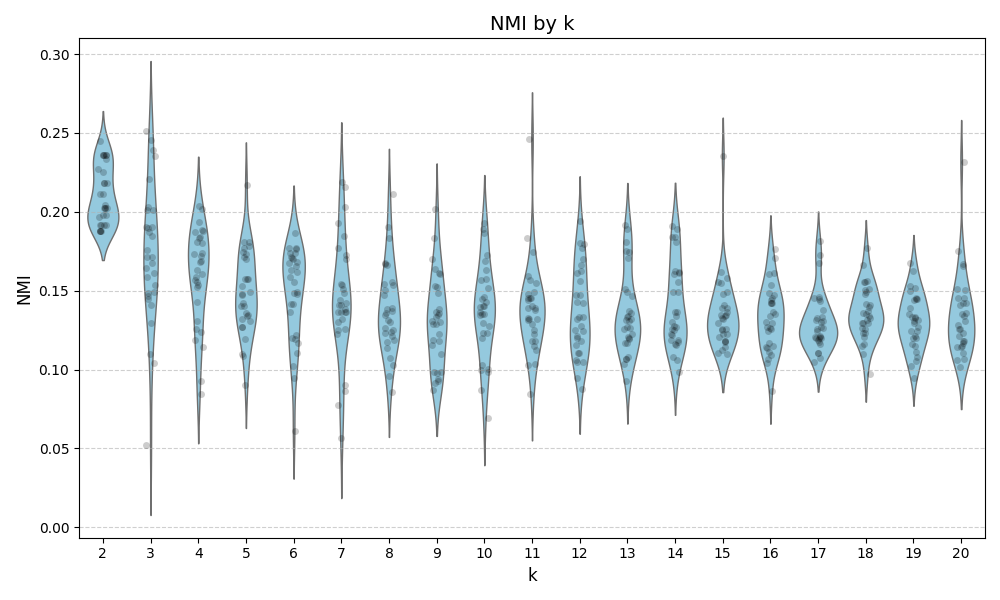
\includegraphics[width=\linewidth]{figures/KMeans/hepatitis_violin_k_vs_NMI.png}
        \caption{Hepatitis NMI}
    \end{subfigure}
    \hfill
    \begin{subfigure}{0.32\textwidth}
        \centering
        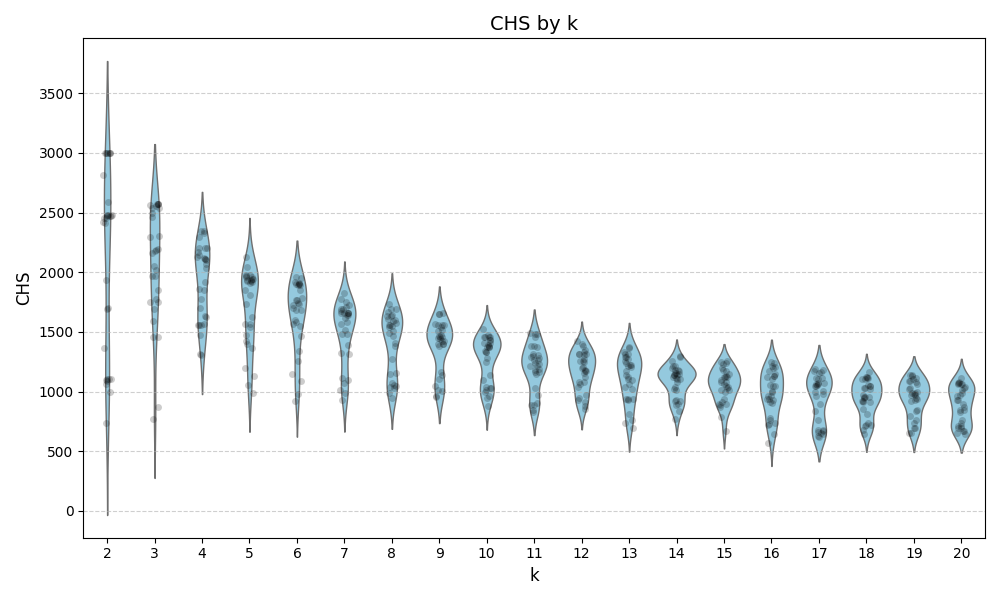
\includegraphics[width=\linewidth]{figures/KMeans/mushroom_violin_k_vs_CHS.png}
        \caption{Mushroom CHS}
    \end{subfigure}
    \hfill
    \begin{subfigure}{0.32\textwidth}
        \centering
        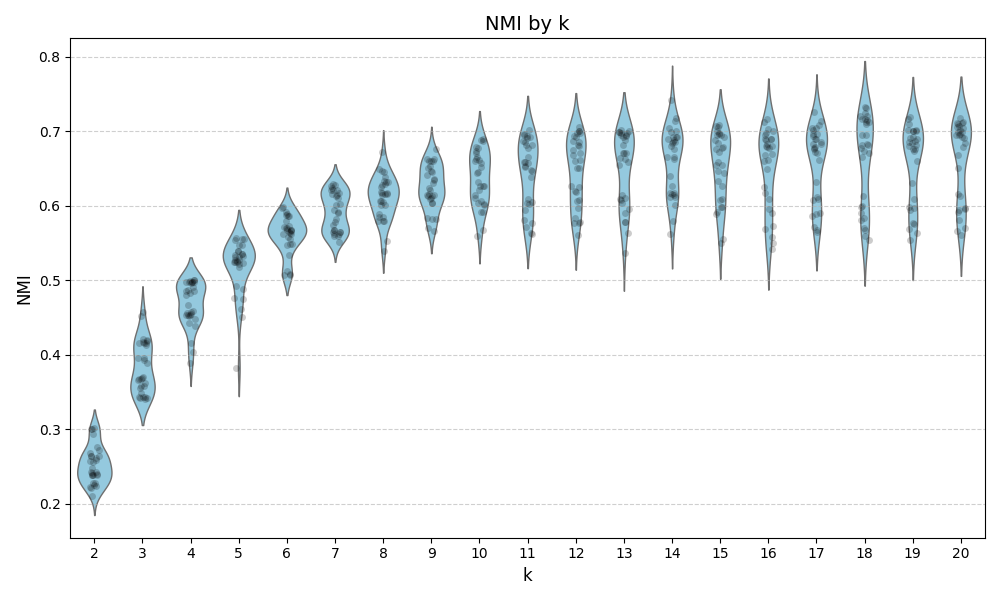
\includegraphics[width=\linewidth]{figures/KMeans/penbased_violin_k_vs_NMI.png}
        \caption{Pen-based NMI}
    \end{subfigure}
    \caption{Violin plots with respect to k for the different datasets}
    \label{fig:kmeans:violin}
\end{figure}

\subsubsection{Best Runs}
For each of the datasets, we extracted the run which achieved the best score for each of the metrics, which results in 5 K-Means algorithm configurations, which we consider to be the 5 best runs for that dataset (in no particular order). A summary of the best runs for the 3 datasets is displayed in Table \ref{tab:kmeans:best_runs}.
\begin{table}[h!]
    \centering
    \begin{tabular}{|c|ccc|ccc|ccc|}
        \hline
                        & \multicolumn{3}{c|}{\textbf{Hepatitis}} & \multicolumn{3}{c|}{\textbf{Mushroom}} & \multicolumn{3}{c|}{\textbf{Pen-based}} \\ \hline
        \textbf{Metric} & \textbf{k} & \textbf{Distance} & \textbf{Value} 
                        & \textbf{k} & \textbf{Distance} & \textbf{Value} 
                        & \textbf{k} & \textbf{Distance} & \textbf{Value} \\ \hline
        ARI            & 2          & manhattan         & 0.37 
                       & 2          & clark         & 0.40 
                       & 14          & euclidean             & 0.64 \\ \hline
        NMI            & 3          & clark             & 0.25 
                       & 15          & clark         & 0.43 
                       & 14          & euclidean         & 0.74 \\ \hline
        DBI            & 20         & euclidean         & 1.40 
                       & 2         & euclidean             & 1.20 
                       & 7         & euclidean         & 1.23 \\ \hline
        Silhouette     & 2          & manhattan         & 0.21 
                       & 2          & euclidean         & 0.28 
                       & 10          & euclidean             & 0.32 \\ \hline
        CHS            & 2          & euclidean         & 36.77 
                       & 2          & euclidean         & 2996.24 
                       & 4          & euclidean         & 3361.02 \\ \hline
    \end{tabular}
    \caption{Metrics with corresponding values, k, and distance metrics for three datasets.}
    \label{tab:kmeans:best_runs}
\end{table}

From these results, we can make some deductions as to which are the best hyperparameter configurations of the K-Means for the 3 datasets:
\begin{enumerate}
    \item \textbf{Hepatitis:} It is again clear that low values of k (2 and 3) typically achieve better scores, which we had already observed before. On the other hand, it is not so clear which of the 3 distance metrics is more appropriate for this dataset, since all of them appear in the top scoring runs.
    \item \textbf{Mushroom:} We can observe once again that k=2 is dominant, probably due to the 2 classes that the dataset has. As for the distance metrics, Euclidean seems to be the most effective, followed by Clark, and Manhattan does not appear to be useful for the properties of this dataset.
    \item \textbf{Pen-based:} In this case, we do not see such a clear predominance of any specific value of k, but there seems to be a trend towards intermediate values, which was to be expected due to the 10 classes of the dataset. In contrast, we do see a constant primacy of the Euclidean distance metric over the rest, that clearly appears to be better at capturing key differences in this dataset than the other two.
\end{enumerate}
Additionally, we can observe that the 2 bigger datasets (Mushroom and Pen-based) have overall better top values of the metrics than the smaller, Hepatitis dataset. In particular, the Pen-based has the best results in all of the metrics except DBI (in which the difference is minimal), which leads us to the conclusion that it is the dataset for which the K-Means clustering algorithm is better suited.

Finally, we display in Figure \ref{fig:kmeans:clusters} the resulting clusters for some of the best runs (one per dataset), after transforming the samples through a PCA with 2 components. Due to the high amount of samples, the Mushroom and Pen-based plots might appear somewhat cluttered, but the clusters can still be identified.

\begin{figure}[H]
    \centering
    \begin{subfigure}{0.32\textwidth}
        \centering
        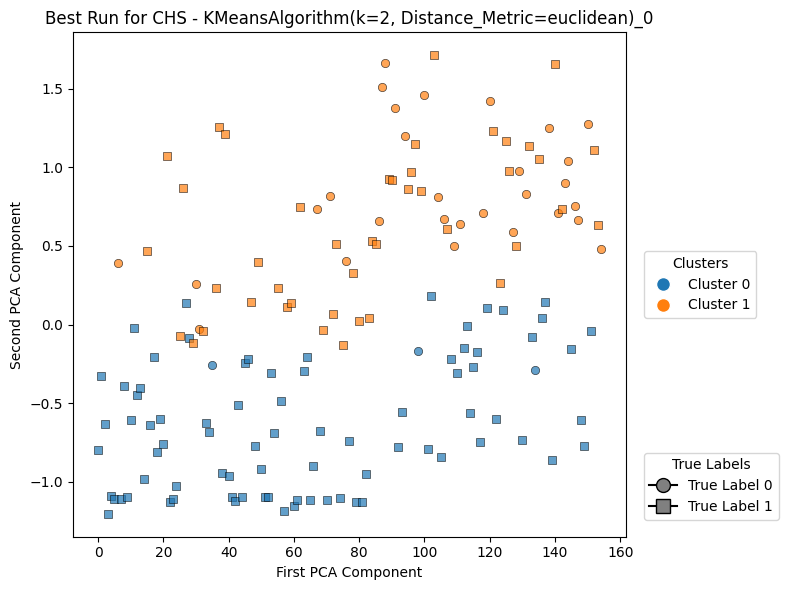
\includegraphics[width=\linewidth]{figures/KMeans/hepatitis_best_run_CHS.png}
        \caption{Hepatitis}
    \end{subfigure}
    \hfill
    \begin{subfigure}{0.32\textwidth}
        \centering
        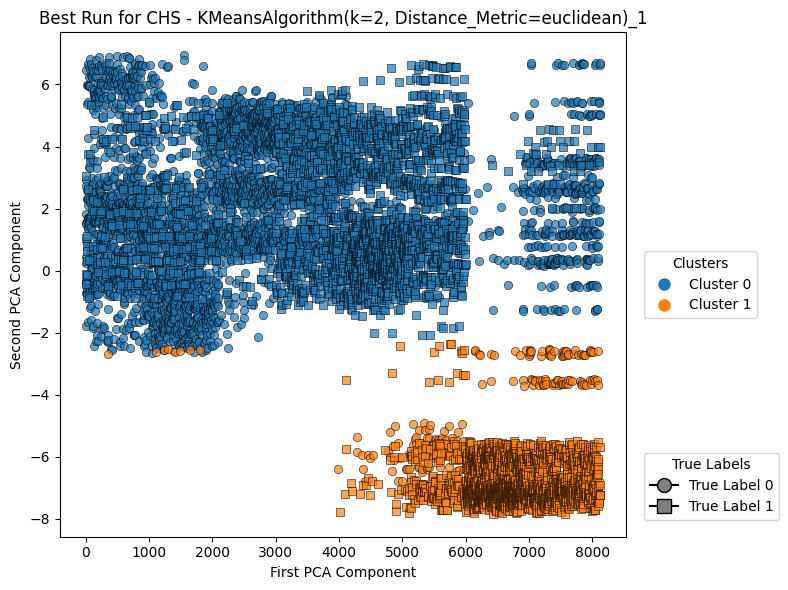
\includegraphics[width=\linewidth]{figures/KMeans/mushroom_best_run_CHS.png}
        \caption{Mushroom}
    \end{subfigure}
    \hfill
    \begin{subfigure}{0.32\textwidth}
        \centering
        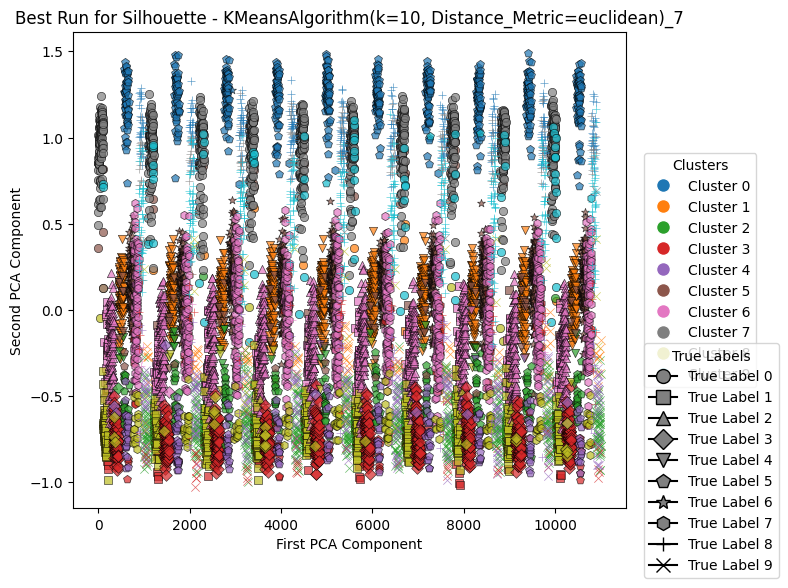
\includegraphics[width=\linewidth]{figures/KMeans/penbased_best_run_Silhouette.png}
        \caption{Pen-based}
    \end{subfigure}
    \caption{Resulting clusters for each dataset (after PCA)}
    \label{fig:kmeans:clusters}
\end{figure}